\section{Phase Screen Realizations and Wave Propagation}
\label{sec:ps_theory}

The amplitude and phase distortions caused by a random ionosphere medium on a wave propagating from a GNSS satellite to a receiver plane is governed by the parabolic wave equation (PWE) \cite{rinoCompactMultifrequencyGNSS2018} \cite{rinoTheoryScintillationApplications2011} \cite{vasylyevModelingIonosphericScintillation2022}.

Considering that the ionospheric irregularities are usually enlongated along the magnectic field line \cite{SizeShapeOrientationOfEquatorialAnomalyScintillations}, we can neglect the distortions caused by the ionosphere medium on the north-south direction for equatorial regions \cite[Section III]{JiaoMultifrequencyScintillationOnGPSSignalsStaticPlatforms2018}. Thus, a continuous scalar form of the PWE is sufficient to describe the interaction of the GNSS propagated signal through the ionosphere and its diffractive pattern seen on the observer plane, which can be given by \cite[Equation 6]{rinoCompactMultifrequencyGNSS2018}:
\begin{align}
    \label{eq:PWE}
    \frac{\partial \psi\left( x, y \right)}{\partial x} = \Theta_{\rho_F} \psi \left( x, y \right) + j k \Delta n \left( x, y \right) \psi \left( x, y \right) \text{.}
\end{align}
where $x$ is the downward direction normal to the ionosphere layer and $y$ is the geomagnectic eastward, $\psi\left( x, y \right)$ is the principal component of the propagated electromagnetic field, $\Theta_{\rho_F} \psi \left( x, y \right)$ represents the free-space propagation, which is related to the diffraction pattern observed in the receiver plane, where the $\Theta_{\rho_F}$ operator is defined in \cite[Equation 7 and 8]{rinoCompactMultifrequencyGNSS2018} and $j k \Delta n \left( x, y \right) \psi \left( x, y \right)$ denotes the refraction of the propagated signal caused by its passage through the ionosphere medium. Furthermore, $k=2\pi f_c/c$ is the transmitted signal wavenumber and $\Delta n\left( x, y \right)$ symbolizes a local pertubation on the refractive index. Figure \ref{fig:propagation_geom} shows the geometric configuration of a GNSS signal oblique propagation.
\begin{figure}
    \centering
    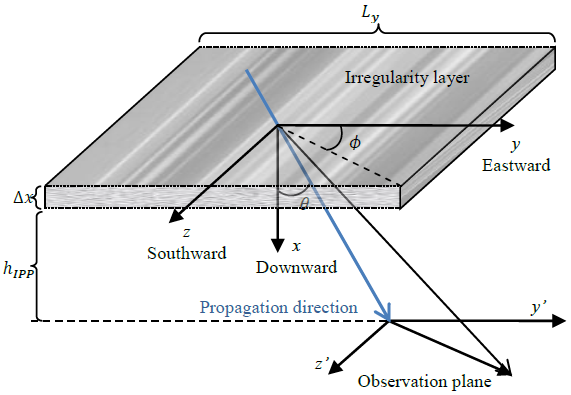
\includegraphics[width=0.45\textwidth]{figures/Propagation Geometry - Yu Jiao.png}
    \caption{Propagation geometry of the scintillation signal. This figure was copied from Figure 2 of \cite{JiaoMultifrequencyScintillationOnGPSSignalsStaticPlatforms2018}}
    \label{fig:propagation_geom}
\end{figure}

A widely adopted solution for the equation \eqref{eq:PWE} is known as the split-step algorithm, which alternates between generating a discrete realization of the phase shift related to the propagated signal refraction in the ionosphere medium and the computation of the free-space propagation effects \cite{rinoTheoryScintillationApplications2011}. In general, to obtain a meaningful scintillation signal, it is necessary to iterate the split-step algorithm through multiple phase screens \cite{vasylyevModelingIonosphericScintillation2022}. However, as was argued in \cite{rinoCompactMultifrequencyGNSS2018}, it is possible to replace the usage of multiple phase screens by a single \textit{equivalent} phase screen for equatorial scintillation events. 

The split-step algorithm can be summarized by the pair of discrete equations \eqref{eq:fft_phase_realization} and \eqref{eq:free_space_propagation} \cite[Equations 1 and 2]{xuTwoparameterMultifrequencyGPS2020}:
\begin{align}
    \label{eq:fft_phase_realization}
    \Psi\left[ 0; n \right] = \sum^{N-1}_{m=0}{\exp\left\{ j \phi\left[ m \right] \right\} \exp\left\{ -2\pi j n m / N \right\}} \text{;}
\end{align}
\begin{align}
    \label{eq:free_space_propagation}
    \psi\left[ x; m  \right] = \frac{1}{N}  \sum^{N-1}_{n=0} \Psi\left[ 0; n \right]
    &\exp \left\{ -j k \left( n \Delta q / k \right)^2 x / 2 \right\} \times \notag \\ 
    \times & \exp\left\{ 2 \pi j n m / N \right\} \text{,}
\end{align}
where $\Psi \left[ 0; n \right]$ represents a $N$-size discrete Fourier transform (DFT) of a complex signal $\exp\left\{ j \phi\left[ m \right] \right\}$ with a unitary amplitude and a phase characterized by the signal $\phi\left[ m \right]$, which is generated from a modeled spectral density function (SDF) with a resolution of discrete samples of $\Delta y$. In addition, $q$ denotes the spatial frequency in the $y$ direction with $\Delta q$ being its resolution.

After substituing the value of $x$ by the Fresnel scale
\begin{align}
    \rho_F = \sqrt{x/k} \text{,}
\end{align}
the equation \eqref{eq:free_space_propagation} can be further simplified as
\begin{align}
    \label{eq:free_space_propagation_simplified}
    \psi\left[ \rho_F; m \right] = \frac{1}{N} \sum_{n=0}^{N-1} \Psi\left[ 0; n \right]
    & \exp \left\{ -j\left( n\Delta q \rho_F \right)^2 /2 \right\} \times \notag \\
    \times & \exp \left\{ 2\pi j n m /N \right\}
\end{align}

As proposed in \cite{rinoCompactMultifrequencyGNSS2018}, a realistic path-integrated phase realization can be obtained from a one-dimensional two-component power law SDF, which can be defined as
\begin{align}
    \label{eq:original_SDF}
    \Phi_{\phi}\left( q \right) = C_p 
    \begin{cases} 
        q^{-p_1}, & q \leq q_0 \\ 
        q_0^{p_2 - p_1} q^{-p_2}, & q > q_0
    \end{cases}
\end{align}
where $q_0$ denotes the spatial wavenumber at which the power-law index change from $p_1$ to $p_2$, and $C_p$ is the turbulence strength \cite[Description below equation 5]{JiaoScintillationOnGPSSignalsForDynamicPlatforms2018}.

It is possible to simplify the equation \eqref{eq:original_SDF} by normalizing the spatial frequency by the fresnel scale, using $\mu = q \rho_F$. With that, we can rewrite the phase SDF as \cite[Equation 6]{JiaoScintillationOnGPSSignalsForDynamicPlatforms2018}
\begin{align}
    P\left( \mu \right) = \Phi_{\phi}\left( q \right) / \rho_F = 
    \begin{cases} 
        U_1 \mu^{-p_1}, & \mu \leq \mu_0 \\ 
        U_2 \mu^{-p_2}, & \mu > \mu_0
    \end{cases}
\end{align}
where $U_1 = C_p \rho_F^{p_1 - 1}$ and $U_2 = C_p \rho_F^{p_1 - 1} \mu_0^{p_2 - p_1}$. It is important to comment here that some papers uses the symbol $C_{pp}$ instead of $U_1$ \cite[Equation 21]{a rinoCompactMultifrequencyGNSS2018}. Therefore, the so-called universal scattering strength $U$ can be defined as \cite[Equation 7]{JiaoScintillationOnGPSSignalsForDynamicPlatforms2018}
\begin{align}
    U =
    \begin{cases}
        C_{pp} = U_1, & \mu_0 \geq 1 \\
        U_2, & \mu_0 < 1
    \end{cases} \text{,}
\end{align}
where $U_2 = U_1 \mu_0^{p_2-p_1}$. With that, we can observe that $U$ is the normalized phase spectral power at $\rho_F$, given that $U \equiv P\left( \mu = 1 \right)$ \cite{Carrano2016OverviewOfTwoComponentPowerLaw}. When $U \ll 1$, the scatter is weak, and when $U \gg 1$, the scatter is strong \cite{Carrano2016OverviewOfTwoComponentPowerLaw}. 

In order to extend the irregularity parameters obtained for a specific frequency band to others, a scaling approach is applied. Since ionospheric scintillation parameters are frequency-dependent, their values for a frequency band $f_2$ are derived by adjusting those from $f_1$ using a frequency ratio factor. This ensures consistency in parameter estimation across different frequencies.

The normalized break wavenumber parameter at a frequency band $f_2$, denoted as $\mu_{0,f_2}$, is scaled from a frequency band $f_1$ using the relation \cite[Equation 17]{JiaoScintillationOnGPSSignalsForDynamicPlatforms2018}:
\begin{equation}
    \label{eq:mu0_extrapolation}
    \mu_{0,f_2} = \mu_{0,f_1} \sqrt{f_1 / f_2}
\end{equation}

Similarly, an extrapolated time-scaling parameter, ${\rho_F / v_{eff}}_{f_2}$, is given by \cite[Equation 18]{JiaoScintillationOnGPSSignalsForDynamicPlatforms2018}:
\begin{equation}
    \label{eq:rhoFveff_extrapolation}
    {\rho_F / v_{eff}}_{f_2} = {\rho_F / v_{eff}}_{f_1} \sqrt{f_1 / f_2}
\end{equation}

Lastly, the universal turbulence strength parameter $U_{f_2}$ is extrapolated from $U_{f_1}$ using the following piecewise relation \cite[Equation 19]{JiaoScintillationOnGPSSignalsForDynamicPlatforms2018}:
\begin{equation}
    \label{eq:U_extrapolation}
    U_{f_2} =
    \begin{cases} 
        U_{f_1} \left(f_1 / f_2\right)^{0.5p_1 + 1.5}, &\mu_{0,f_1} \geq 1, \mu_{0,f_2} \geq 1 \\
        U_{f_1} / \mu_{0,f_1}^{p_2-p_1} \left( f_1 / f_2 \right)^{0.5 p_1 + 1.5}, & \mu_{0,f_1} < 1, \mu_{0,f_2} \geq 1 \\
        U_{f_1} \left( \mu_{0,f_2} / \mu_{0,f_1} \right)^{p_2 - p_1} \left(f_1 / f_2\right)^{0.5 p_1 + 1.5}, & \mu_{0,f_1} < 1, \mu_{0,f_2} < 1
    \end{cases}
\end{equation}

It is important to emphasize here that the equations \eqref{eq:mu0_extrapolation}, \eqref{eq:rhoFveff_extrapolation} and \eqref{eq:U_extrapolation} are derived based on weak scintillation theory and serve as approximations in strong scattering conditions \cite{Rino1979WeakScatter}.

A comprehensive analysis of the two-component power law spectra can be found in \cite{Carrano2016OverviewOfTwoComponentPowerLaw}. This work underpinned the importance of understanding the physical meaning of this kind of spectral model, which also nests a widely used one-component power law model \cite{CarranoBrazil2012}. The two-component power law model can be modeled in such manners that it captures the electron density statistical properties of the inner and outer scales that defines the complete ionosphere structure. With that, this spectra is well-suited for modeling weak and strong signal scattering caused on the ionosphere medium.

A Statistically equivalent phase screen realization $\overline{\phi}\left[ m \right]$ can be obtained by imposing $P\left( \mu \right)$ on a complex Gaussian random variable $\eta\left[ n \right] \sim \mathcal{C N}\left( 0, 1 \right)$ with the Hermitian and the white noise properties \cite{rinoCompactMultifrequencyGNSS2018}
\begin{align}
    \eta\left[ n \right] = \text{mod}\left( \eta^*\left[ N \right], N \right) \text{,} \\
    \mathbb{E}\left\{ \eta\left[ n \right] \eta^{*}\left[ n' \right] \right\} = \delta\left[ n-n' \right] \text{,}
\end{align}
respectively, where $mod\left( \cdot \right)$ denotes the modulus operator and $E\left\{ \cdot \right\}$ represents the expectation. Thus, we have
\begin{align}
    \label{eq:phase_screen_realization}
    \overline{\phi}\left[ m \right] = \sum_{n=0}^{N-1} \sqrt{P(n\Delta \mu) \Delta \mu / (2\pi)} \, \eta\left[ n \right] \exp\{-2 \pi j n m / N\} \text{.}
\end{align}
It is worthy to clarify that this equation represents an inverse discrete Fourier Transform (IDFT). Note here that the term $1/N$ that commonly appears in a IDFT is related to $\Delta \mu$ in this equation, which in its part is related to the variable of integration of the IDFT. Please refer to \cite[Section 6.1]{vasylyevModelingIonosphericScintillation2022} and \cite[Section 2.2.4]{rinoTheoryScintillationApplications2011} for further details on the generation of phase realizations based on a defined SDF.

The split step algorithm can be implemented considering equations \eqref{eq:idft_phase_realization_simplified} and \eqref{eq:free_space_propagation_simplified} using a phase realization generated by equation \eqref{eq:phase_screen_realization} as \cite[Equations 9 and 10]{JiaoScintillationOnGPSSignalsForDynamicPlatforms2018}
\begin{align}
    \label{eq:idft_phase_realization_simplified}
    \Psi\left[ 0; n \right] = \sum^{N-1}_{m=0}{\exp\left\{ j \overline{\phi}\left[ m \right] \right\} \exp\left\{ -2\pi j n m / N \right\}} \text{,}
\end{align}
\begin{align}
    \label{eq:post-prop_scint_field}
    \psi\left[ \rho_F; m \right] = \frac{1}{N} \sum_{n=0}^{N-1} \Psi\left[ 0; n \right]
    & \exp \left\{ -j\left( n\Delta \mu \right)^2 /2 \right\} \times \notag \\
    \times & \exp \left\{ 2\pi j n m /N \right\} \text{.}
\end{align}

Furthermore, conversion of the complex field from the space domain to the time domain can be achieved by using a effective scan velocity $v_{eff}$, such that $y\left[ 1 \right] - y\left[ 0 \right] = v_{eff} \left( t\left[ 1 \right] - t\left[ 0 \right] \right)$ \cite[Equation 11]{JiaoMultifrequencyScintillationOnGPSSignalsStaticPlatforms2018}. The effective scan velocity is computed using knowledge of the velocity of the ionospheric piercing point (IPP), the ionosphere mean drift velocity (Which ranges between 25 m/s and 125 m/s \cite{SizeShapeOrientationOfEquatorialAnomalyScintillations} \cite{Wang2017IonoDriftHighLatitude}) and the anisotropy coefficients related to the expected shapes of the ionosphere turbulent media. The reader is referred to \cite[Section 4]{JiaoScintillationOnGPSSignalsForDynamicPlatforms2018} and \cite[Chapter 4]{rinoTheoryScintillationApplications2011} for further details on the computation of $v_{eff}$.

It is worthy to comment for completness here that there are many ways of computing the IPP location for mutually known receiver position and satellite orbit. A comparative study of the most used methods can be found in \cite{Prol2017_Comparative_Study}. 

In addition, it is possible to observe at the file \textit{.../Libraries/PropGeomCalc/PropGeomCalc.m} available at the github repository \url{https://github.com/cu-sense-lab/gnss-scintillation-simulator_2-param} uses the fixed values for the anistropy coefficients $a=50$, $b=1$ and $\gamma_b = 0$. In order to avoid compromising the feasibility of the assumption that the PWE only depends on the eastward direction $y$, i.e., that the change in the refractive index in the southward direction $z$ is negligible, it is better not to change these values, either for the weak and strong scattering cases. The reader is referred to \cite{Vasylyev2024WeakScatterAnisotropy} for details on the ionospheric turbulences anisotropy. 

Considering \cite[Equation 2-14]{harrington2001time} and \cite[The text before equation 26]{rinoCompactMultifrequencyGNSS2018}, we may state the following relation:
\begin{align}
    q &= 2 \pi f_D / v_{eff} \big|_{\times \ \rho_F} \ \therefore \notag \\
    \therefore \ \Delta \mu &= 2 \pi \Delta f_D \rho_F / v_{eff} \text{,}
\end{align}
where $f_D$ represents the Doppler frequency shift related to the effective scan velocity, and $\Delta f_D = 1/\left( N \Delta t \right)$ correponds to the resolution of the samples of the Doppler frequency, where $\Delta t$ denotes the sampling time of the scintillation complex field simulation. It is important to emphasize here that $f_D$ is not directly related to the phase shift caused by receiver-satellite line-of-sight range dynamics. For further detailing of the meaning of $f_D$, please refer to \cite[Text before equation 5]{carrano2017maximum}.

Summarizing, a GNSS complex field scintillation time series can be generated by specifying the irregularity parameters $U$, $p_1$, $p_2$ and $\mu_0$, the time scaling factor $\rho_F / v_{eff}$, which depends only on the satellite-ionosphere-receiver propagation geometry and the sampling parameters $\Delta t$ and $N$. The next section will review how prior studies have proposed to estimate these parameters.